\section{Design}
\label{sec:design}

Section IV of the authors' IoTDI 2017 paper already gave a high-level description of namespace design, trust management and local rendezvous in Flow.
This section does a review of each piece, and then describes the corresponding mechanisms in NDN-IoT framework.

\subsection{Naming and Identity}
\label{sec:naming}

% Design: namespace
In Flow, data from the IoT \textit{things} used by the application are named using three namespaces:
\begin{itemize}
\item \emph{Application namespace}: a local namespace for publishing and accessing application data, e.g., gyroscope readings needed to control the environment; 
\item \emph{Device namespace:} a local namespace for publishing device identity certificates and metadata;\footnote{Device metadata could include information about devices and their capabilities as well as bindings to application names.}
\item \emph{Manufacturer namespace}: a global namespace created by the IoT device vendors and for trust bootstrapping.
\end{itemize}

% One question I commonly get from people in and outside the team: why different namespaces?
This separation of namespaces is reflected in section VI.A of cite:iotdi-2016 paper: naming application data separately from the device that produces it, since typically when a consumer in the application requests a piece of data, it cares about the received data being authentic and useful, not necessarily from where or which device this data is sent out.

Fig.~\ref{fig:flow-namespace} shows an example of the Flow namespace.
In addition to these three namespaces which names devices, things and their data, note the \textit{discovery} branch under the local root prefix, which is used for device rendezvous and for application prefix discovery.
Details of its functionality are described later.

\begin{figure*}[!t]
\centering
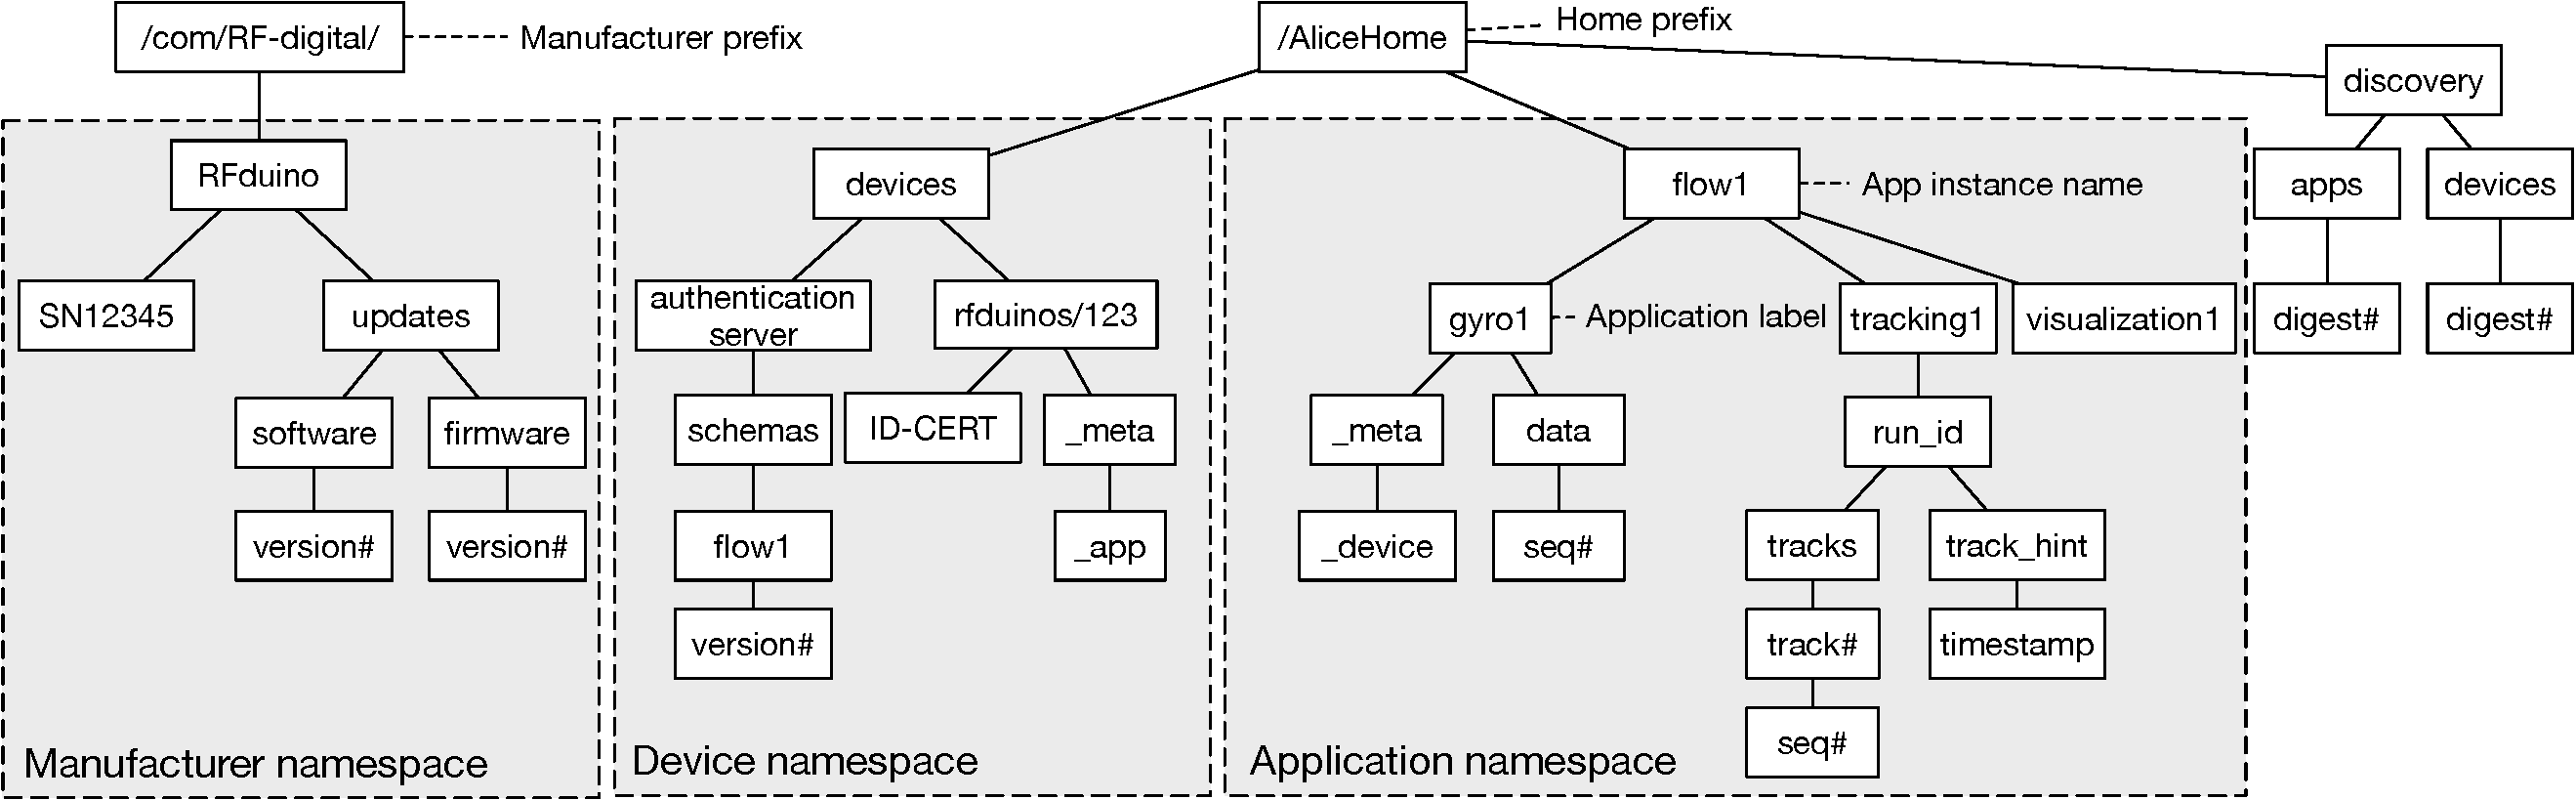
\includegraphics[width=0.95\textwidth]{flow-namespace.pdf}
\caption{Example namespace within the home environment where Flow is deployed.}
\label{fig:flow-namespace}
\end{figure*}

The device and application namespaces both have as their root a home prefix that is either context-dependent (e.g., \ndnName{/AliceHome} as in Fig.~\ref{fig:flow-namespace}) or globally reachable (e.g., \ndnName{/att/ucla/dorm1/301}).

The application namespace starts with a unique instance name (e.g., \ndnName{/AliceHome/flow1}) created by the application at installation. 
Data produced by each component is named under an application label configured by the developer (e.g. \ndnName{/AliceHome/flow1/tracking1}). 
The application label also contains a metadata subtree containing the device name that serves this data (e.g. \ndnName{/AliceHome/flow1/tracking1/_meta/_device}).

Devices publish their local identity certificates under the device namespace (e.g., \ndnName{/AliceHome/devices}).
They also publish metadata information in the \ndnName{_meta/_app} branch under the device identity prefix to list the application data prefixes they are publishing under. 
The device namespace of an AS also contains the trust schema of currently active applications. 
Schema and trust relationship details are described later in this section.

In this work we added an additional \textit{manufacturer namespace} that is independent from the local root namespace, since we envision that manufacturers will have globally unique names for their products used during bootstrapping, over-the-air updates, and similar processes. 
Manufacturers publish their own certificates under this globally unique prefix so that the devices can authenticate the data coming from the vendors such as software/firmware updates and service notifications.\footnote{Reachability of data in this prefix is not addressed here but can be accomplished through encapsulation supported by the home router, for example.}
In Flow, all devices are configured with vendor-provided identity names and profiles in their initial provisioning, before being connected to the home network.
These names are used during onboarding, in the name of the first command interest that the AS sends out to add the device to the home network.
This process is described in more detail in the coming subsection.

NDN-IoT framework interface supports the separation of application namespace and device namespace, and application developers can supply arbitrary names to both, or get a configured default device names obtained from device onboarding process. 
An example of the interface is later described in Section~\ref{sec:implementation-ndn-iot}.

\subsection{Trust Management}
\label{sec:trust-management}

Flow demonstrates a multi-step process for trusting new devices in a home IoT network and enabling their data to be used in an application. 
First, a device is assigned a device-level name and added to the trust hierarchy for things in the home. 
Then, it is configured with one or more application-level names for its data, and these names are added to application trust hierarchies. 
Finally, the device is configured to respond to requests in application namespaces. 

The AS acts as the trust anchor. 
It can be coordinated with but does not depend on a remote cloud services.
While the devices and users may have public identities outside the home environment, they all need to obtain local identities that are certified by the AS before they can start interacting with other local entities.

The process of establishing a trust relationship between a new device and the home through the AS is similar to the Bluetooth pairing process.
To bootstrap a new device, the user---or a configuration application on his/her behalf---provides a shared secret and a local device name.
The shared secret may be a device barcode, identity communicated by NFC, or simply a PIN number. 

The AS sends a command Interest to the device, signed using a key derived from the shared secret, to ask that it generate a public/private key pair associated with the device's new name on the local network.
The device replies with a Data packet containing an identity certificate request, also signed by the shared secret.
The AS generates the identity certificate based on this request.
The device, now part of the trust hierarchy, can advertise its services or participate in an application over the local network.
This process is illustrated in Fig.~\ref{fig:flow-bootstrap}.

\begin{figure}[!t]
\centering
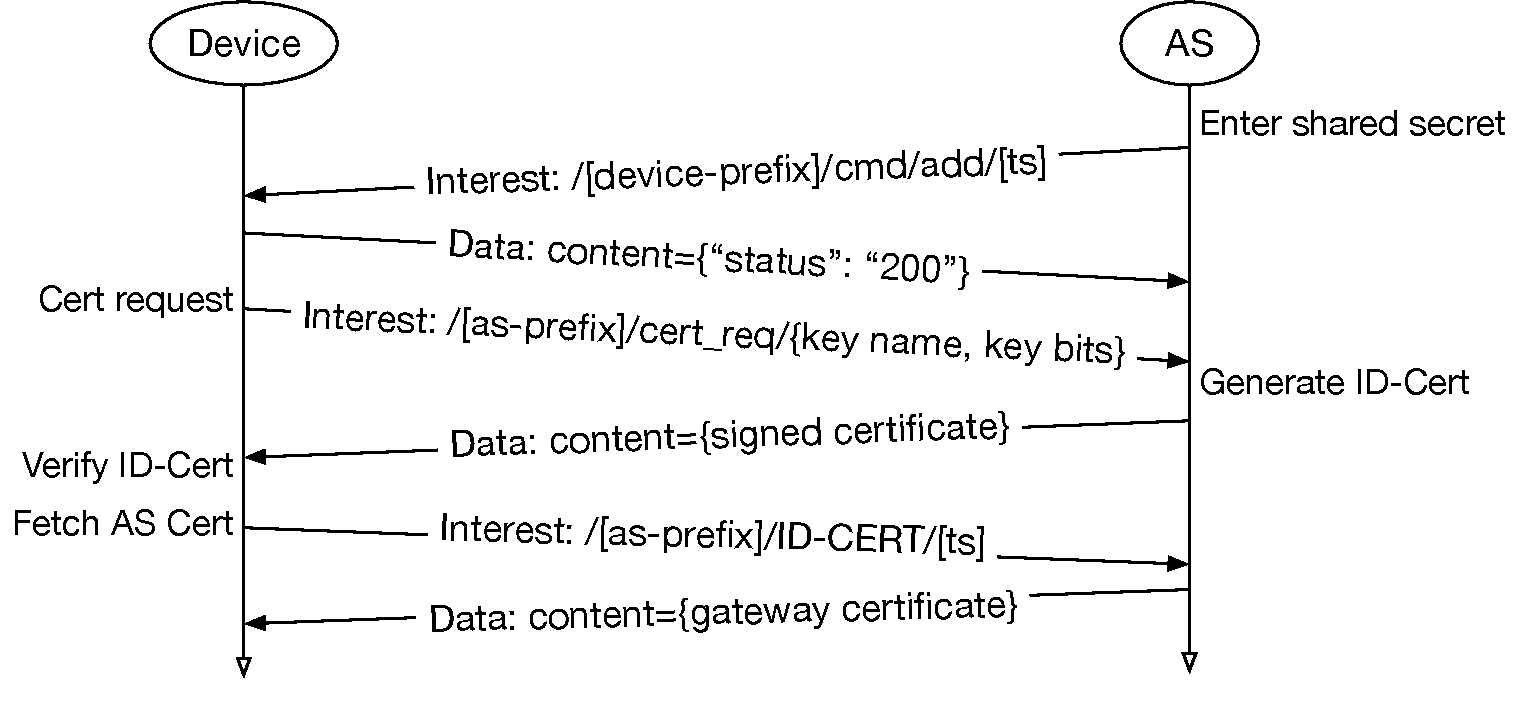
\includegraphics[width=0.95\columnwidth]{add-device-sequence.pdf}
\caption{Bootstrap trust relationship for new device.}
\label{fig:flow-bootstrap}
\end{figure}

Applications like Flow are ``installed'' in a similar way to devices, with the AS signing both identity certificates and trust schema for the application.
The application's trust schema expresses \textit{what devices identities are authorized to publish under what application prefixes} and is published as a normal Data object on the local NDN network. 
For example, in Fig.~\ref{fig:flow-namespace} \ndnName{flow1} is a specific Flow instance and \ndnName{schema} branch contains the trust schema of this instance.
The schema name includes a monotonic version number at the end, so when there is a change in the schema a newer version is published.
The technical details of how to specify a trust schema are described in~\cite{trust-schema}.

% Design: trust - application producer authorization
When a device that produces data is installed, it sends a command Interest to the AS that includes the application prefix it intends to publish under and its own local identity.
If the request to publish data in the home network is granted, the AS will update the trust schema with the authentication rules for data published by this device.
The rule binds a device identity with the application prefixes it's authorized to publish under.
\footnote{This binding addresses potential collision in application labels--for example, by default the AS does not authorize a second device to publish under an application namespace claimed by another.}
Schematized trust enables fine-grained control over what devices can publish what data for which application instances.
Consumer devices fetch the latest trust schema over the network via NDN and follow the rules to authenticate the data packets published in the network.

The producer authorization process, as well as an example of the resulting trust relationship, is shown in Fig.~\ref{fig:flow-app-authorization-trust-relationship}, in which the AS signs a device identity, and the device signs a piece of application data it publishes.

\begin{figure}[!t]
\centering
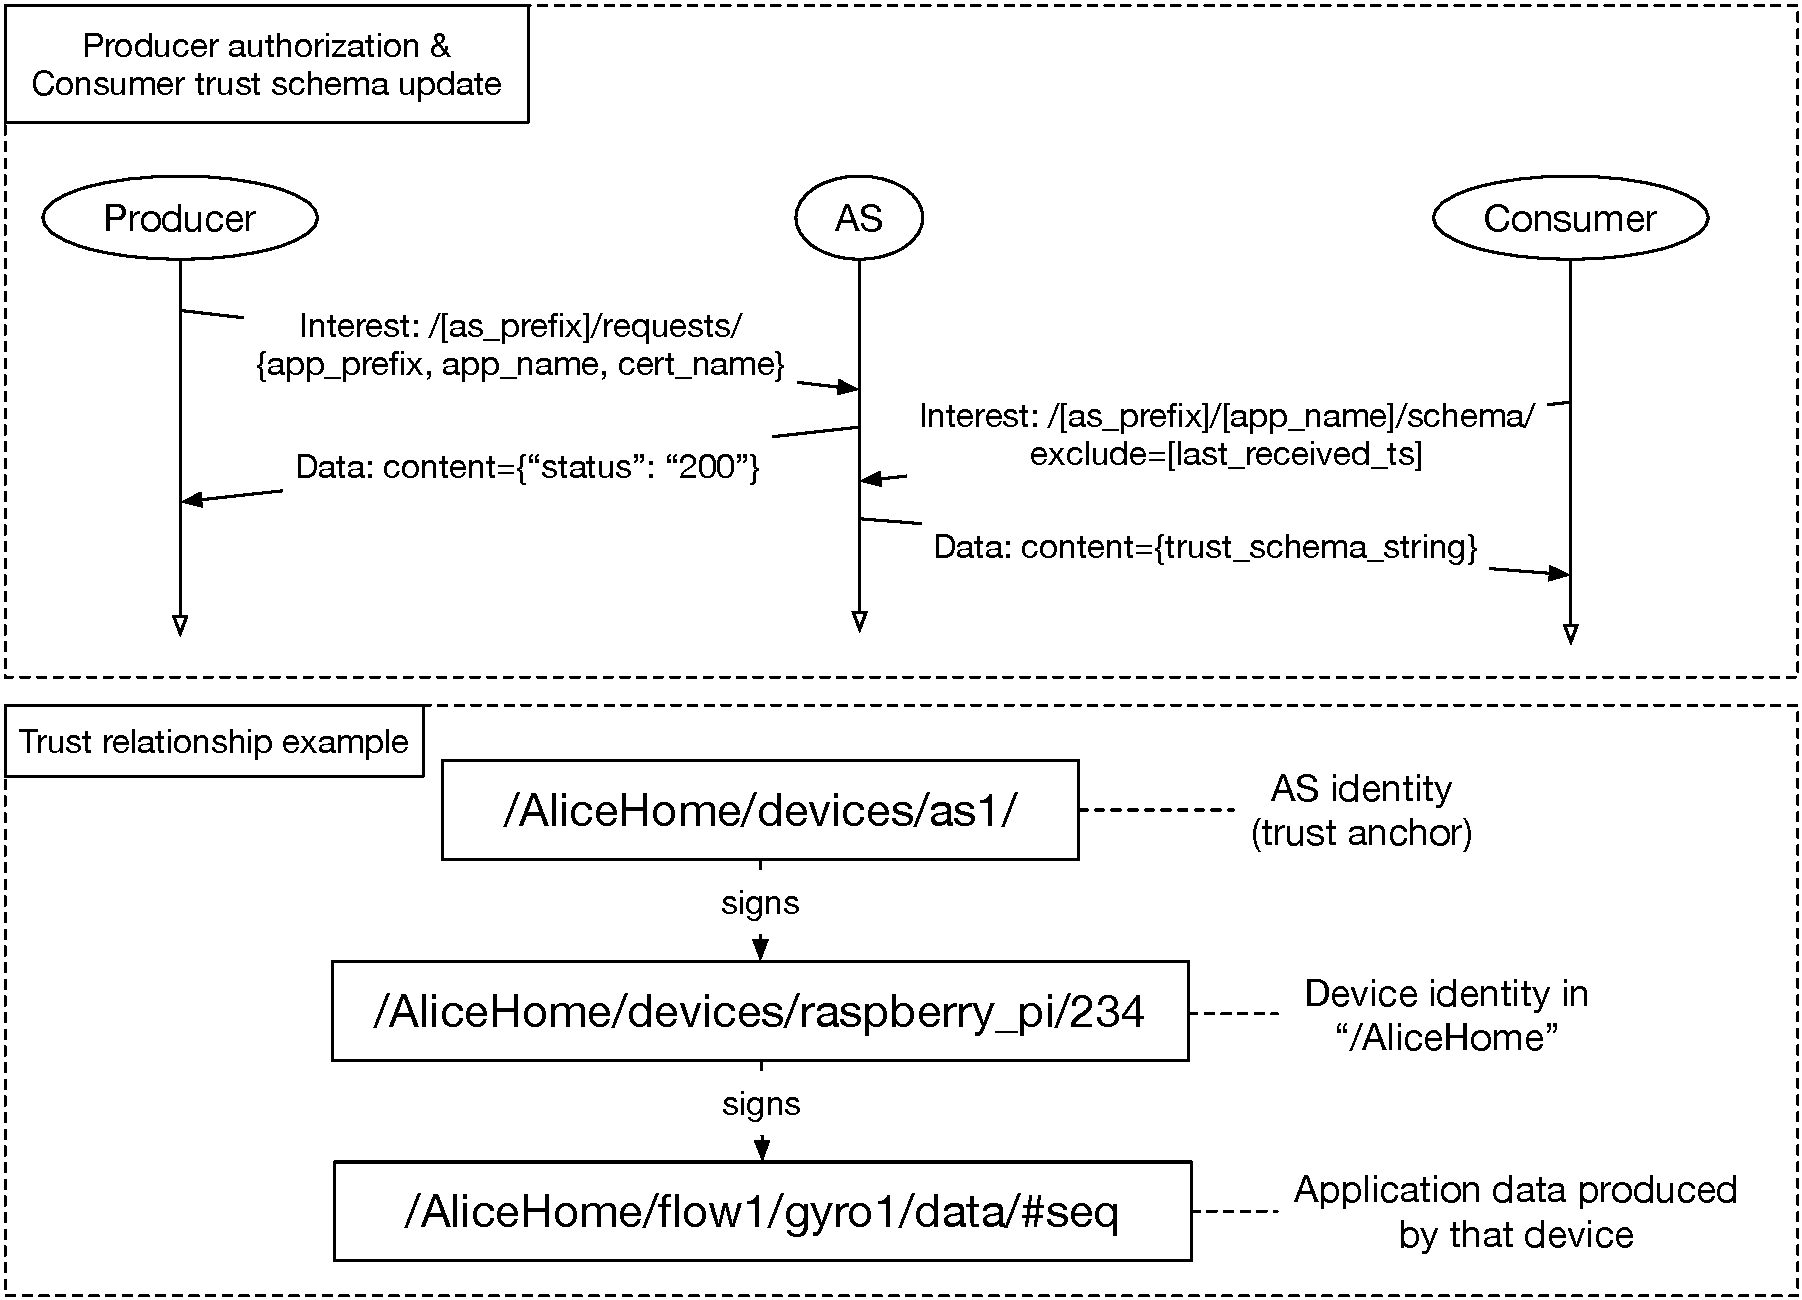
\includegraphics[width=0.95\columnwidth]{authorize-producer-consumer.pdf}
\caption{Schematized trust between producers and consumers.}
\label{fig:flow-app-authorization-trust-relationship}
\end{figure}

NDN-IoT framework provides an example implementation of AS, client scripts for device onboarding, and an interface for producers to request publishing authorization and consumers to keep track of the application instance's trust schema.
An example trust schema built by the AS, and application API calls are described in Section~\ref{sec:implementation-ndn-iot}.

\subsection{Rendezvous}
\label{sec:rendezvous}

Flow also demonstrates a name-based, distributed rendezvous mechanism for devices and applications to discover each other over NDN.
As described in the previous section, The key idea is to synchronize the set of device and application names (called the \textit{rendezvous dataset}) across nodes in the network that are interested in learning about them.
The synchronization process utilizes a ChronoSync~\cite{chronosync} recovery-like protocol to synchronize prefixes of active devices under the \ndnName{/AliceHome/discovery/devices} namespace.

Name discovery is performed independently on each device by lookups in the local copy of the rendezvous dataset. 
The device sends a multicast Interest with the digest of its local rendezvous dataset attached to the name. 
Receivers of this interest, upon seeing a different digest, will reply in a Data packet with its own set of names. 
The device can then obtain the name prefix from the set difference, and follow the namespace structure described in~\ref{sec:naming} to construct Interests for fetching the certificates and metadata, which will bootstrap high-level service communication.

An example discovery process is shown in Fig.~\ref{fig:flow-discovery-process}, in which \textit{Device1} discovers name \ndnName{/c} from the network and then fetches data from it.

\begin{figure}[!t]
\centering
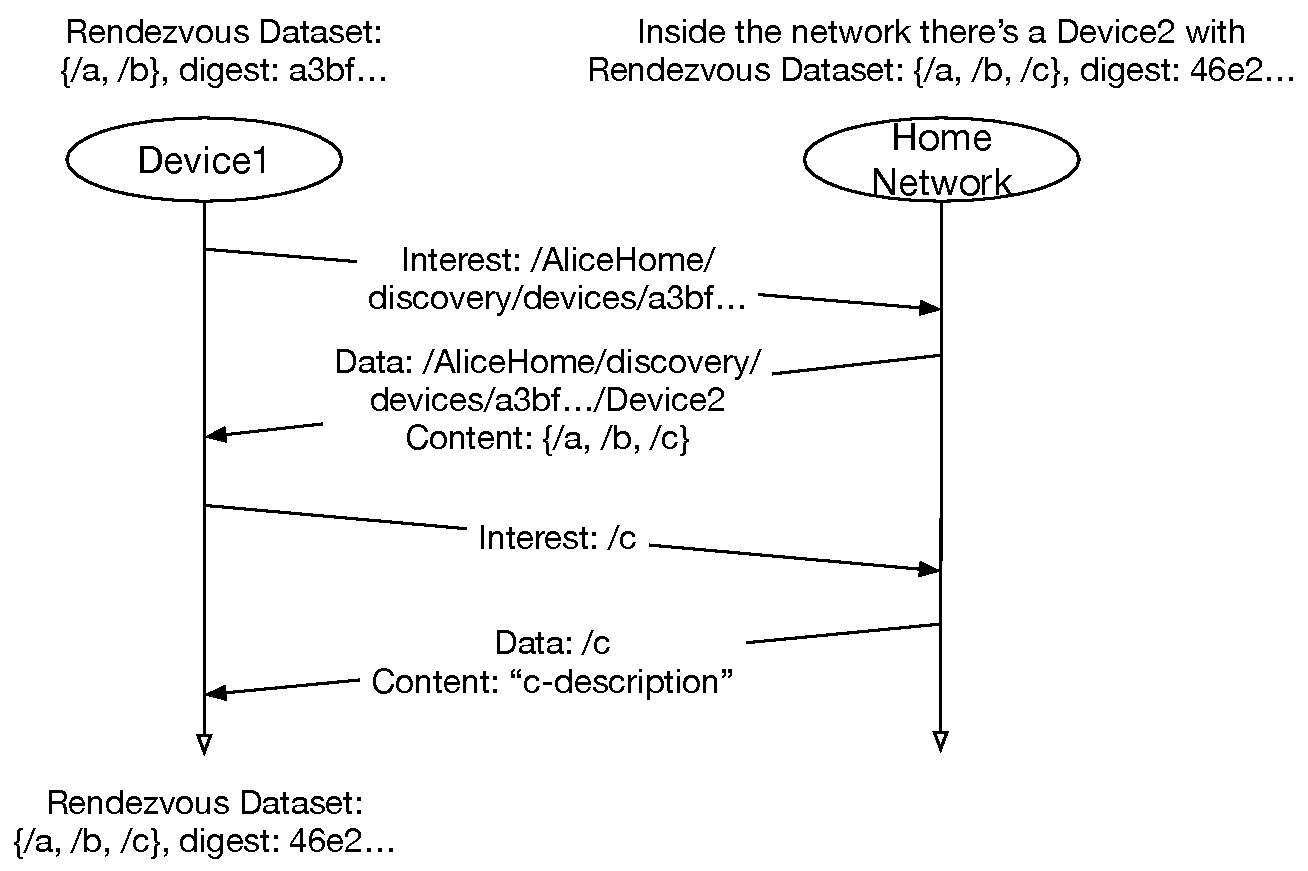
\includegraphics[width=0.95\columnwidth]{flow-discovery-process.pdf}
\caption{Example of Flow discovery process.}
\label{fig:flow-discovery-process}
\end{figure}

NDN-IoT provides an implementation of this distributed discovery mechanism, whose interface is further described in Section~\ref{sec:implementation-ndn-iot}.

\subsection{Application-level pub/sub}

Pub/sub is identified as a common pattern in IoT applications in \cite{ndn-iot}.
To facilitate application development NDN-IoT framework implements application-level pub/sub in two commonly used namespaces: 

\emph{Timestamp namespace}, in which producer publishes time series data whose last name component is a timestamp. 
The framework uses outstanding interest and range exclusion between $<$\emph{Any, previously received timestamp}$>$ to fetch the next piece of content.
\footnote{If exclusion filter is deprecated, the framework could switch to using a manifest of data names for consuming in a timestamp namespace}

\emph{Sequence-number namespace}, in which data's last name is a sequence number. 
The framework pipelines interest with the sequence numbers of the next few data packets in this namespace.

The workflow of both is shown in Figure~\ref{fig:application-level-pub-sub}.

\begin{figure}[!t]
\centering
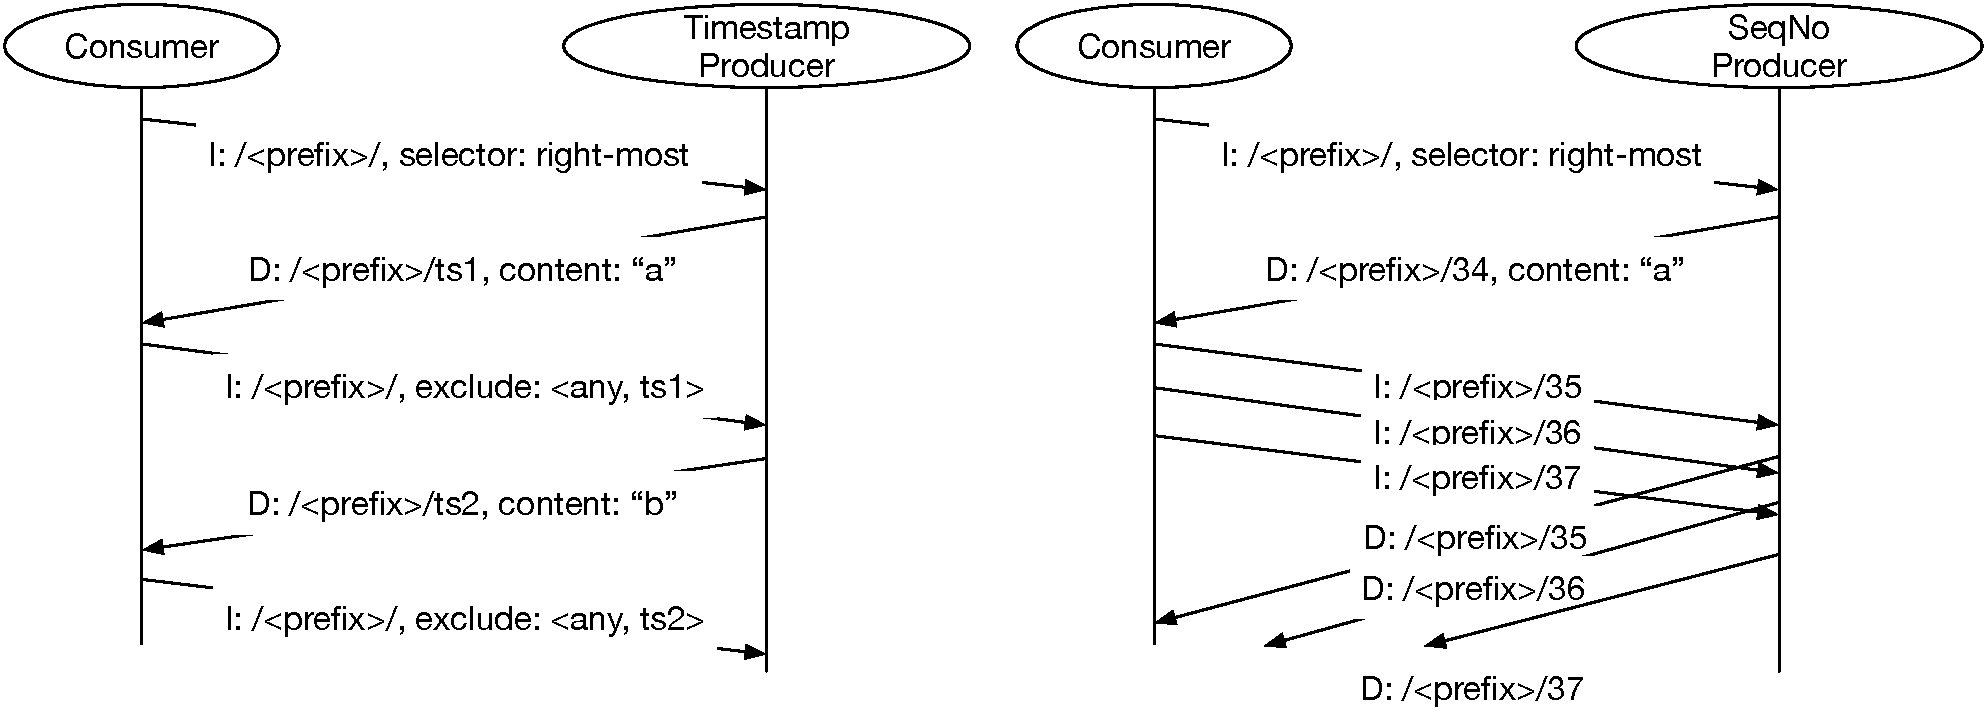
\includegraphics[width=0.95\columnwidth]{app-pubsub-namespaces.pdf}
\caption{Application-level pub/sub in NDN-IoT framework.}
\label{fig:application-level-pub-sub}
\end{figure}

\subsection{Supporting constrained devices}
\label{sec:constrained-device}

Flow involves producers running on constrained devices not powerful enough to perform asymmetric signing operations quickly, and may not have a forwarder implementation dedicated to their platforms. 
For those devices we introduce a helper that bridges them to the NDN home network.

In the framework, the pairing between constrained device and its helper is established using a shared secret key, manually put into both devices (not unlike the device onboarding step between a device and the AS).
The helper then generates a public/private key pair on behalf of the constrained device to be associated with the latter's device identity.
The constrained device may run a simple publisher which pushes data (signed by the shared secret) to the helper, and the helper repackages the data and signs the data using constrained device's private key, and then publishes the data on the home network.

An example of this pattern is described in Section~\ref{sec:implementation-ndn-iot}.

